\documentclass{article} % For LaTeX2e
\usepackage{iclr2026_conference,times}

\usepackage{hyperref}
\usepackage{url}

\usepackage{threeparttable}
\usepackage{xspace}
\usepackage{epsfig}
\usepackage{graphicx}
\usepackage{amsmath,amsfonts}
\usepackage{amssymb}
\usepackage{amsthm}
\usepackage[misc]{ifsym}
\usepackage{amsfonts}
\usepackage{bm}
\usepackage{bbm}
\usepackage{array}
\usepackage{multicol}
\usepackage{multirow}
\usepackage{enumitem}
\usepackage{nccmath}
\usepackage{pifont}% http://ctan.org/pkg/pifont
\usepackage{multirow}
\usepackage{array}
\usepackage{adjustbox}
\usepackage{enumitem}
\usepackage{caption}
\usepackage{booktabs}
\usepackage{ragged2e}
\usepackage[ruled,vlined,linesnumbered]{algorithm2e}
\usepackage{dblfloatfix}
\usepackage{ifsym}
\newcommand{\cmark}{\ding{51}}%
\newcommand{\xmark}{\ding{55}}%


\newcommand{\graytext}[1]{{\textcolor[RGB]{128,138,135}{#1}}}

\newcommand{\boldparagraph}[1]{\vspace{0.2cm}\noindent{\bf #1}}

\newcommand{\onedot}{.\xspace}
\def\eg{\emph{e.g}\onedot} \def\Eg{\emph{E.g}\onedot}
\def\ie{\emph{i.e}\onedot} \def\Ie{\emph{I.e}\onedot}
\def\cf{\emph{c.f}\onedot} \def\Cf{\emph{C.f}\onedot}
\def\etc{\emph{etc}\onedot} \def\vs{\emph{vs}\onedot}
\def\wrt{w.r.t\onedot} \def\dof{d.o.f\onedot}
\def\etal{\emph{et al}\onedot}

\makeatletter
\newcommand{\algorithmfootnote}[2][\footnotesize]{%
  \let\old@algocf@finish\@algocf@finish% Store algorithm finish macro
  \def\@algocf@finish{\old@algocf@finish% Update finish macro to insert "footnote"
    \leavevmode\rlap{\begin{minipage}{\linewidth}
    #1#2
    \end{minipage}}%
  }%
}
\makeatother

\usepackage[utf8]{inputenc} % allow utf-8 input
\usepackage[T1]{fontenc}    % use 8-bit T1 fonts
\usepackage{nicefrac}       % compact symbols for 1/2, etc.
\usepackage{microtype}      % microtypography
\usepackage{wrapfig}
\definecolor{deepgreen}{RGB}{0,128,0}
\usepackage{appendix}
\def\thename{VADv2\xspace}


\title{VADv2：基于概率规划的端到端矢量化自动驾驶}

% Authors must not appear in the submitted version. They should be hidden
% as long as the \iclrfinalcopy macro remains commented out below.
% Non-anonymous submissions will be rejected without review.

\author{
    \quad \quad \ \ Bo Jiang$^{1, *,\diamond}$, \quad Shaoyu Chen$^{2,*}$, \quad Hao Gao$^{1,\diamond}$, \quad Bencheng Liao$^{1,\diamond}$, \\
    \textbf{\quad \quad \ \ \ Qian Zhang$^{2}$, \quad Wenyu Liu$^{1}$, \quad Xinggang Wang$^{1,\textrm{\Letter}}$} \\
    \\
    \quad \quad \ \ \ $^1$华中科技大学 \quad $^2$地平线机器人 \\
    \quad \quad \ \ \ \texttt{\{bjiang, ghao, bcliao, liuwy, xgwang\}@hust.edu.cn} \\
    \quad \quad \ \ \ \texttt{\{shaoyu.chen, qian01.zhang\}@horizon.auto}
}

% The \author macro works with any number of authors. There are two commands
% used to separate the names and addresses of multiple authors: \And and \AND.
%
% Using \And between authors leaves it to \LaTeX{} to determine where to break
% the lines. Using \AND forces a linebreak at that point. So, if \LaTeX{}
% puts 3 of 4 authors names on the first line, and the last on the second
% line, try using \AND instead of \And before the third author name.

\newcommand{\fix}{\marginpar{FIX}}
\newcommand{\new}{\marginpar{NEW}}

\iclrfinalcopy % Uncomment for camera-ready version, but NOT for submission.
% Chinese support (auto-injected)
\usepackage{xeCJK}
\setCJKmainfont{Noto Serif CJK SC}[ItalicFont=AR PL UKai TW MBE]
\setCJKsansfont{Noto Sans CJK SC}
\setCJKmonofont{Noto Sans CJK SC}
\raggedbottom
\renewcommand{\figurename}{图}
\renewcommand{\tablename}{表}
\renewcommand{\abstractname}{摘要}
\renewcommand{\refname}{参考文献}
\begin{document}


\maketitle

\begin{abstract}
从大规模驾驶演示中学习类人驾驶策略前景广阔，但规划的不确定性和非确定性本质使其充满挑战。现有基于学习的规划方法遵循确定性范式直接回归动作，难以应对不确定性问题。本文提出了一种用于端到端自动驾驶的概率规划模型，称为VADv2。我们采用概率场函数对从动作空间到概率分布的映射进行建模。由于规划动作空间是高维连续时空空间且难以处理，我们首先将规划动作空间离散化为一个大型规划词表，然后将规划词表标记化为规划令牌。规划令牌与场景令牌交互，输出动作的概率分布。大规模驾驶演示被用于监督该分布。VADv2在CARLA Town05基准上取得了最先进的闭环性能，显著优于现有方法，并且在最近的Bench2Drive基准上也处于领先地位。我们进一步在NAVSIM和基于大规模3D高斯泼溅的基准上提供了全面的评估，证明了其在实际应用中的有效性。代码开源地址：\textcolor{magenta}{\url{https://github.com/hustvl/VAD}}。
\end{abstract}

\let\thefootnote\relax\footnotetext{$^*$同等贡献。$^\diamond$ 工作于地平线机器人实习期间完成。$^\textrm{\Letter}$ 通讯作者。}

\section{引言}
% \vspace{-1mm}
\label{sec:introduction}

端到端自动驾驶是当前重要的研究课题。真实场景中的大规模人类驾驶演示易于获取，从这些丰富的演示中学习类人驾驶策略用于车辆控制极具前景。然而，规划的不确定性和非确定性本质使得从驾驶演示中提取驾驶知识充满挑战。为说明这种不确定性，图~\ref{fig:intro}展示了两个场景并解释如下。1) 跟随另一辆车：人类驾驶员表现出多种合理的驾驶操作，如保持当前车道或变道超车。2) 与对向车辆交互：人类驾驶员面临两种可能的驾驶操作，即让行或超车。从统计角度看，动作（包括时机和速度）高度随机，受众多无法精确建模的潜在因素影响。

现有基于学习的规划方法~\citep{vad, uniad, thinktwice, transfuser, mile, roach}遵循确定性范式直接回归动作。回归目标在~\citep{vad, uniad, thinktwice, transfuser}中为未来轨迹，在~\citep{mile, roach}中为控制信号（加速度和转向）。这种范式假设驾驶场景与动作之间存在确定性关系，但事实并非如此。人类驾驶行为的方差导致回归目标的模糊性。特别是当可行解空间非凸时，\ie，存在多个可行解（见图~\ref{fig:intro}），确定性建模可能无法正确处理此类情况并产生中间动作，带来潜在的安全风险。


\begin{wrapfigure}{r}{0.55\textwidth}
\centering
\vspace{-0.3mm}
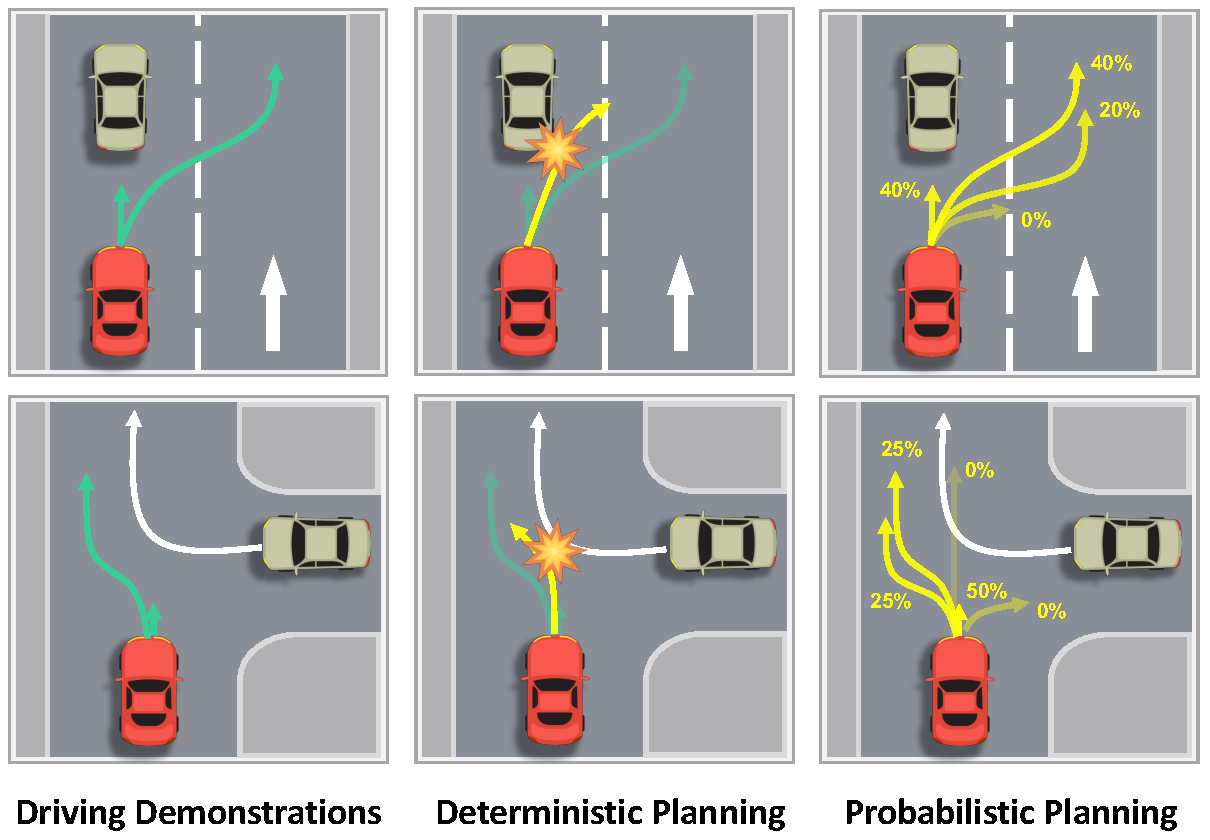
\includegraphics[width=0.55\textwidth, height=0.4\textwidth]{fig/intro.pdf}
% \vspace{0.2mm}
\caption{规划中存在不确定性。驾驶场景与动作之间不存在确定性关系。确定性规划无法对此类不确定性进行建模，尤其在可行解空间非凸的情况下。\thename{}基于概率规划，从大规模驾驶演示中学习场景条件下的动作概率分布。}
\label{fig:intro}
\vspace{-3mm}
\end{wrapfigure}


本文提出概率规划以应对规划的不确定性。我们将规划策略建模为场景条件下的非平稳随机过程，公式化为$p(\bm{a} | \bm{o})$，其中$\bm{o}$是驾驶场景的历史和当前观测，$\bm{a}$是候选规划动作。与确定性规划相比，概率规划对规划中的不确定性更为鲁棒，能够对非凸可行解空间进行建模，从而实现更准确、更安全的规划。

我们采用概率场函数对从规划动作空间到概率分布的映射进行建模。由于动作空间是高维连续时空空间且难以处理，我们首先将规划动作空间离散化为一个大型规划词表，然后将规划词表标记化为规划令牌。规划令牌与场景令牌交互，输出动作的概率分布。大规模驾驶演示被用于监督该分布。

概率规划还有两个额外优势。第一，不同于确定性规划需要基于场景信息回归最优动作，概率规划对每个动作与驾驶场景之间的相关性进行建模，只需对不同动作进行排序并采样高分动作。这种建模方式更简单。此外，概率规划在推理阶段具有灵活性，输出多模态规划结果，易于与基于规则和基于优化的规划方法结合。由于对动作空间整体分布进行建模，可以灵活地向规划词表中添加其他候选动作并评估。

基于概率规划，本文提出端到端驾驶模型VADv2，以流式方式接收环视图像序列输入，对传感器数据和规划动作空间进行标记化，输出动作的概率分布，并采样一个动作控制车辆。仅使用相机传感器，VADv2在CARLA Town05基准上取得了最先进的闭环性能，显著优于现有方法，同时在最近的Bench2Drive基准上也处于领先地位。在NAVSIM和基于3DGS的基准上也展现出强大的规划性能。\thename{}以完全端到端方式稳定运行，甚至不需要基于规则的包装器作为后处理步骤来避免违规。

\vspace{-0.5mm}
本文贡献总结如下：
\vspace{-0.5mm}
\begin{itemize}[leftmargin=12pt]
    \item 提出概率规划以应对规划的不确定性和非确定性本质。设计概率场来映射从动作空间到概率分布的关系，并从大规模驾驶演示中学习动作分布。
    \item 基于概率规划，提出了\thename{}——一个端到端驾驶模型，将传感器数据和规划动作空间标记化进行交互，输出动作的概率分布，并采样一个动作控制车辆。
    \item \thename{}在多个基准的闭环和开环设置下均取得了最先进的规划性能。丰富的闭环仿真和真实部署结果验证了其在车辆控制中的有效性和稳定性。
\end{itemize}


\vspace{-1mm}
\section{相关工作}
\vspace{-1mm}
\boldparagraph{感知。} 感知是实现自动驾驶的第一步，驾驶场景的统一表示有利于与下游任务的无缝集成。鸟瞰图（Bird's Eye View, BEV）表示近年来已成为通用策略，能够有效编码场景特征并进行多模态数据融合。LSS~\citep{philion2020lss}是一项开创性工作，通过显式预测图像像素的深度来实现透视视图到BEV的变换。而BEVFormer~\citep{li2022bevformer}则通过设计空间和时间注意力机制避免了显式深度预测。后续工作~\citep{li2022bevdepth, StreamPETR}持续优化时序建模和BEV变换策略。在矢量化建图方面，HDMapNet~\citep{li2022hdmapnet}通过后处理将车道分割转换为矢量地图。VectorMapNet~\citep{liu2022vectormapnet}以自回归方式预测矢量地图元素。MapTR~\citep{liao2022maptr, maptrv2}引入排列等价和层次化匹配策略，显著提升了建图性能。LaneGAP~\citep{lanegap}引入车道图的路径化建模。


\boldparagraph{运动预测。} 运动预测旨在预测其他交通参与者的未来轨迹，辅助自车做出合理的规划决策。传统运动预测方法利用历史轨迹和高精度地图等输入预测未来轨迹~\citep{gao2020vectornet, liu2021mmtrans}。而最近的端到端方法~\citep{gu2022vip3d, jiang2022pip}联合执行感知与运动预测。部分工作~\citep{hu2021fiery, zhang2022beverse}将未来运动表示为稠密的占用和流场，另一些工作~\citep{gu2022vip3d, jiang2022pip}则预测智能体级别的多模态轨迹。另一类工作将轨迹预测重新定义为分类问题而非回归任务。Trajeglish~\citep{philion2023trajeglish}引入K-disk采样构建紧凑的单步运动词表，与k-means相比离散化误差更小。MotionLM~\citep{seff2023motionlm}将每个单步动作分解为纵向和横向分量，并应用轴向对齐的均匀量化。虽然这种单步建模实现了紧凑表示和小词表，但迭代推理可能导致误差累积并产生违反物理约束的轨迹。相比之下，VADv2中每个动作令牌表示完整轨迹，确保物理可行的运动基元，实现无误差累积的一次性规划。


\boldparagraph{规划。} 基于学习的规划最近展现出巨大潜力，得益于其数据驱动的特性以及随着数据量增加而带来的令人印象深刻的性能提升。早期尝试~\citep{codevilla2019exploring, prakash2021multi}采用完全黑盒的思想，直接用传感器数据预测控制信号。但这种策略缺乏可解释性且难以优化。此外，有大量研究将强化学习与规划相结合~\citep{roach, gao2025rad}，在闭环仿真环境中自主探索驾驶行为。模仿学习~\citep{chekroun2021gri, hu2022stp3, ma2025leapvad}是另一个研究方向，模型学习专家驾驶行为以获得良好的规划性能并形成接近人类的驾驶风格。

UniAD~\citep{uniad}集成多个感知和预测任务以增强规划性能。VAD~\citep{vad}探索矢量化场景表示在规划中的潜力并摆脱稠密地图。Diffusion Planner~\citep{zheng2025diffusionplanner}通过迭代扩散联合预测自车和其他智能体的运动，但依赖真值感知和高精度地图。DiffusionDrive~\citep{liao2025diffusiondrive}通过截断扩散加速去噪过程；然而有限且预定义的轨迹锚点可能限制生成质量，增加锚点数量又引入额外的计算开销。GoalFlow~\citep{xing2025goalflow}将规划分解为目标点选择以及通过流匹配生成轨迹，但依赖单一目标点可能影响轨迹多样性，且手工设计的轨迹选择规则限制了泛化性和可扩展性。


\begin{figure*}[ht]
\centering
% \vspace{1mm}

\includegraphics[width=0.98\textwidth]{fig/framework.pdf} % Reduce the figure size so that it is slightly narrower than the column.
\vspace{2mm}
\caption{\textbf{\thename{}的整体架构。} \thename{}以流式方式接收多视角图像序列输入，对传感器数据和规划动作空间进行标记化，输出动作的概率分布，并采样一个动作控制车辆。大规模驾驶演示和场景约束被用于监督预测分布。}
\label{fig:framework}
\end{figure*}


\boldparagraph{大语言模型与自动驾驶。} 近期研究探索了LLM与自动驾驶的结合~\citep{languagempc, drivegpt4}。一类工作利用LLM通过问答进行驾驶场景理解和评估~\citep{driving-with-llms, sima2024drivelm}。另一种方法更进一步，直接利用LLM进行规划~\citep{drivemlm, wang2024drivecot}。然而，当前基于LLM的规划方法不可避免地受到推理速度的限制，这制约了其在自动驾驶应用中实时部署的实用性。\thename{}从GPT~\citep{achiam2023gpt4}中汲取灵感来应对不确定性问题，该问题同样存在于语言建模中。在给定特定上下文下，下一个词是非确定的，LLM从大规模语料库中学习上下文条件下的下一个词的概率分布，并从分布中采样一个词。受LLM启发，\thename{}将规划策略建模为场景条件下的非平稳随机过程。\thename{}对动作空间进行离散化生成规划词表，基于大规模驾驶演示近似概率分布，并在每一时间步从分布中采样一个动作来控制车辆。


\section{\thename{}}
\label{sec:method}

\thename{}的整体框架如图~\ref{fig:framework}所示。\thename{}以流式方式接收多视角图像序列输入，将传感器数据转换为场景令牌嵌入，输出动作的概率分布，并采样一个动作控制车辆。大规模驾驶演示和场景约束被用于监督预测分布。


\subsection{场景编码器}

\thename{}使用场景编码器将传感器数据转换为实例级令牌嵌入$E_{\rm scene } \in \mathbb{R}^{M \times D}$以显式提取高层信息，其中$M$是场景令牌的数量，$D$是特征维度。具体而言，$E_{\rm scene}$包含四类场景令牌：地图令牌、智能体令牌、交通元素令牌和图像令牌。

\boldparagraph{BEV编码器。} 首先使用BEV编码器~\citep{li2022bevformer}将多视角图像特征从透视视图变换为BEV，生成BEV空间中的特征图。该特征图作为学习实例级地图和智能体特征的基础。

\boldparagraph{地图令牌。} 引入一组地图令牌~\citep{maptrv2}从BEV特征图中学习驾驶场景的矢量化地图元素，包括车道中心线、车道分隔线、道路边界和人行横道。

\boldparagraph{智能体令牌。} 此外，采用一组智能体令牌~\citep{vad}来预测交通参与者的运动信息，包括位置、朝向、尺寸、速度和未来轨迹。

\boldparagraph{交通元素令牌。} 交通信号在规划中也起着至关重要的作用。在CARLA中考虑两种类型的交通信号：交通灯和停止标志。骨干网络提取的前视图图像特征通过MLP进一步编码为交通元素令牌，随后用于预测交通信号的状态。

\boldparagraph{图像令牌。}
除上述实例级令牌外，前视图图像特征也被用作图像令牌。这些图像令牌为规划提供更稠密的场景特征，捕捉丰富的信息以补充实例级令牌。

地图令牌、智能体令牌和交通元素令牌通过相应的监督信号进行监督，确保它们显式编码相应的高层信息。此外，导航信息和自车状态也通过MLP编码为嵌入$(E_{\rm navi}, E_{\rm state})$。总之，场景编码器将稀疏的传感器数据转换为更紧凑的高层场景特征$(E_{\rm scene}, E_{\rm navi}, E_{\rm state})$，为后续的规划模块奠定基础。

\subsection{概率规划}
本文提出概率规划以应对规划的不确定性。将规划策略建模为场景条件下的非平稳随机过程，公式化为$p(\bm{a} | \bm{o})$，其中$\bm{o}$是观测到的场景信息，$\bm{a}$是动作，表示为未来规划轨迹的路径点序列：

\begin{equation}
\bm{o} = (E_{\rm scene}, \ E_{\rm navi}, \ E_{\rm state}), \ \ \bm{a} =(x_{1}, \ y_{1}, \ x_{2}, \ y_{2}, \ldots, \ x_{T}, \ y_{T}).
\end{equation}

$T$是路径点数量。每个路径点$(x_i, y_i)$对应一个未来时间戳$t_i$。


\begin{wrapfigure}{r}{0.5\textwidth}
\vspace{-4.5mm}
\LinesNotNumbered
\begin{algorithm}[H]
\SetAlgoLined
\DontPrintSemicolon
\SetNoFillComment
\footnotesize
\KwIn{规划动作集 $\mathcal{S}$，规划词表大小 $N$}
\KwOut{规划词表 $\mathcal{V}$}
初始化: $\mathcal{V} \leftarrow \emptyset$ \;
\For{$i=1$ to $N-1$}{
\If{$\mathcal{V} == \emptyset$}{
    从 $\mathcal{S}$ 中随机选择一个动作 $\bm{a}$ \;
    $\mathcal{V} \leftarrow \mathcal{V} \cup \{\bm{a}\}$ 将动作加入规划词表 \;
    $\mathcal{S} \leftarrow \mathcal{S} \setminus \{\bm{a}\}$ 将动作从规划动作集中移除 \;
    }
$max\_dis=0$\;
\For{{轨迹} $\bm{a}$ in $S$}{
    $dis = \textbf{calculate\_distance}(\bm{a}, \mathcal{V})$ \;
    \If{$dis > max\_dis$}{
        $max\_dis = dis$ \;
        $\hat{\bm{a}} = \bm{a}$ 更新当前最远轨迹 \;
    }
}
$\mathcal{V} \leftarrow \mathcal{V} \cup \{\hat{\bm{a}}\}$ \;
}
返回: $\mathcal{V}$
\caption{规划词表采样算法。}
% \vspace{-4mm}
\label{algo:vocab}
\end{algorithm}
\captionsetup{labelformat=empty}
\caption{$\textbf{calculate\_distance}$计算动作$\bm{a}$的终点与集合$\mathcal{V}$中所有动作终点之间的距离，并返回这些距离中的最小值作为结果。}
\vspace{-5mm}
\end{wrapfigure}


基于大规模驾驶演示来近似规划动作空间的概率分布，并在每个时间步从分布中采样一个动作来控制车辆。


规划动作空间是高维连续时空空间且难以处理。因此，将其离散化为一个大型规划词表$\mathcal{V}=\{\bm{a}^i\}^N$，其中$N$是词表大小。具体而言，收集驾驶演示中的所有规划动作作为规划动作集$\mathcal{S}$，并采用最远轨迹采样（Furthest Trajectory Sampling）选择$N$个代表性动作作为规划词表。词表采样算法如算法~\ref{algo:vocab}所示。$\mathcal{V}$中的每个规划动作均采样自驾驶演示，因此自然满足自车的运动学约束，这意味着当动作转换为控制信号（转向、油门和制动）时，控制信号值不会超出可行范围。默认情况下，$N$设为4096。

假设概率$p(\bm{a})$相对于$\bm{a}$是连续的且对$\bm{a}$的微小扰动不敏感，\ie，$\lim_{\Delta \bm{a} \to 0} {\left( p(\bm{a})   -  p(\bm{a}+\Delta \bm{a}) \right)} = 0$。受NeRF~\citep{nerf}的启发（其在5D空间上建模连续辐射场），我们采用概率场来建模从动作空间到概率分布的连续映射。

具体而言，首先将每个动作（轨迹路径点）编码为高维规划令牌嵌入$E(\bm{a})$：


\begin{equation}
\begin{aligned}
& E(\bm{a}) = \bigl(\Gamma(x_{i}), \ \Gamma(y_{i})\bigr)_{i=1}^{T}, \
\Gamma(\mathrm{pos}) = \bigl(\gamma(\mathrm{pos}, \ j)\bigr)_{j=0}^{L-1}, \\
& \gamma(\mathrm{pos}, \ j) = \bigl(\cos(\mathrm{pos}/{10000}^{2\pi j/L}), \ \sin(\mathrm{pos}/{10000}^{2\pi j/L})\bigr).
\end{aligned}
\end{equation}

$\Gamma$是一个编码函数，将每个坐标从$\mathbb{R}$映射到高维嵌入空间$\mathbb{R}^{2L}$，并对轨迹$\bm{a}$的每个坐标值分别应用。$\rm pos$表示位置（指路径点的$x$或$y$坐标）。使用这些函数将连续坐标映射到更高维空间，以更好地近似更高频率的场函数。

然后，级联Transformer解码器$\phi$与场景信息$E_{\rm scene}$交互，并结合导航信息$E_{\rm navi}$和自车状态$E_{\rm state}$，预测每个动作的概率：

\begin{equation}
\begin{aligned}
    & p(\bm{a}) = \sigma({\rm MLP (\phi}(E(\bm{a}), \ E_{\rm scene}) + E_{\rm navi} +  E_{\rm state})). \\
    % & q=E(\bm{a}), k=v=E_{\rm scene}.\\
\end{aligned}
\end{equation}

$\sigma$是sigmoid函数。在Transformer解码器$\phi$中，$E(\bm{a})$作为查询，$E_{\rm scene}$作为键和值。$E(\bm{a})$、$E_{\rm navi}$、$E_{\rm state}$以及MLP的输出具有相同的维度（$1\times D$）。


% \vspace{-2mm}
\subsection{训练}
使用三种监督信号训练\thename{}：分布损失、冲突损失和场景令牌损失。

\boldparagraph{分布损失。} 从大规模驾驶演示中学习概率分布。使用KL散度最小化预测分布与数据分布之间的差异：

\begin{equation}
\mathcal{L}_{\rm distribution} =  D_{\rm KL}(p_{\rm data} || p_{\rm pred}) = \sum_{\bm{a}\in\mathcal{V}}   p_{\rm data}(\bm{a}) \cdot \log \frac{p_{\rm data}(\bm{a})}{p_{\rm pred}(\bm{a})},
\end{equation}

$p_{\rm data}(\bm{a})$通过驾驶演示中的出现频率估计。由于$p_{\rm data}(\bm{a})$是固定的，$p_{\rm data}(\bm{a}) \cdot \log p_{\rm data}(\bm{a})$是常数可以省略。因此，最小化KL散度等价于优化交叉熵损失：

\begin{equation}
\mathcal{L}_{\rm distribution} = - \sum_{\bm{a}\in\mathcal{V}}  p_{\rm data}(\bm{a}) \cdot \log p_{\rm pred}(\bm{a}).
\label{loss_distribution}
\end{equation}

对于演示中的每一帧，从规划词表中选择与真值动作L2距离最小的动作作为最佳匹配动作，赋予标签1，其他所有动作赋予0。在所有帧上，动作$\bm{a}$的出现频率$p_{\rm data}(\bm{a})$通过统计每个动作被选为最佳匹配的次数并除以总帧数来估计。这种建模方式类似于大语言模型中使用的标准公式——真值令牌标记为1，其余为0，用交叉熵损失最小化预测分布与经验分布之间的差异。


\boldparagraph{冲突损失。} 驾驶场景约束被用于帮助模型学习重要的驾驶先验知识并正则化预测的动作分布。具体而言，如果规划词表中的某个动作与其他智能体的真值未来运动或道路边界发生冲突，则将其视为负样本，并施加相应的损失以降低其概率：

\begin{equation}
\begin{aligned}
\mathcal{L}_{\rm conflict}
&= \sum_{\bm{a}\in\mathcal{V}}  \mathbbm{1}_{\rm conflit}(\bm{a}) \cdot \log p_{\rm pred}(\bm{a}).\\
\end{aligned}
\end{equation}
$\mathbbm{1}_{\rm conflit}(\bm{a})$为指示函数，当$\bm{a}$发生冲突时值为1，否则为0。

\boldparagraph{场景令牌损失。} 地图、智能体和交通元素令牌通过相应的监督信号进行监督，确保它们显式编码相关的高层信息。

地图令牌的损失与MapTRv2~\citep{maptrv2}相同。采用$\textit{l}_1$损失计算预测地图点与真值地图点之间的回归损失，Focal损失用作地图分类损失。

智能体令牌的损失由检测损失和运动预测损失组成~\citep{vad}。$\textit{l}_1$损失用作回归损失以预测智能体属性（位置、朝向、尺寸等），Focal损失用于预测智能体类别。对于每个与真值智能体匹配的智能体，预测$K$条未来轨迹，并使用最终位移误差（minFDE）最小的轨迹作为代表性预测。然后计算该代表性轨迹与真值轨迹之间的$\textit{l}_1$损失作为运动回归损失。此外，Focal损失被用作多模态运动分类损失。

交通元素令牌由两部分组成：交通灯令牌和停止标志令牌。一方面，将交通灯令牌送入MLP预测交通灯状态（黄、红、绿）以及该交通灯是否影响自车。另一方面，将停止标志令牌也送入MLP预测停止标志区域与自车之间的重叠。Focal损失用于监督这些预测。最终损失可表示为：

\begin{equation}
\vspace{-1mm}
\mathcal{L} =  \mathcal{L}_{\rm distribution} + \mathcal{L}_{\rm conflict} + \mathcal{L}_{\rm token}.
\vspace{-1mm}
\end{equation}


\subsection{推理}
在闭环推理中，从分布中获取驾驶策略是灵活的。直观上，在每个时间步采样概率最高的动作，并使用PID控制器将选中的动作转换为控制信号（转向、油门和制动）。

在实际应用中，存在更鲁棒的策略来充分利用概率分布。一个良好的实践是：采样Top-K动作作为候选，采用基于规则的包装器过滤候选，并使用基于优化的后求解器进行细粒度轨迹优化。此外，动作的概率反映了端到端模型的置信度，可以作为在传统规则规划控制和基于学习的规划控制之间切换的判断条件。


\begin{table*}
\caption{Town05 Long基准上的闭环评估结果。}
\vspace{-3mm}
\begin{center}
\renewcommand{\tabcolsep}{9pt}
\centering
\resizebox{0.98\linewidth}{!}{
\begin{tabular}{lccccc}
\toprule
方法 & 参考文献 & 模态 & DS $\uparrow$ & RC $\uparrow$ & IS $\uparrow$ \\
\midrule
Transfuser~\citep{transfuser} & TPAMI'22 & C+L & 31.0 & 47.5 & 0.77 \\
ThinkTwice~\citep{thinktwice} & CVPR'23 & C+L & 70.9 & 95.5 & 0.75 \\
DriveAdapter+TCP~\citep{driveadapter} & ICCV'23 & C+L & 71.9 & 97.3 & 0.74 \\
DriveMLM~\citep{drivemlm} & arXiv'23 & C+L & 76.1 & 98.1 & 0.78 \\
\midrule
Roach~\citep{roach} & ICCV'21 & C & 41.6 & 96.4 & 0.43 \\
ST-P3~\citep{hu2022stp3} & ECCV'22 & C & 11.5 & 83.2 & - \\
MILE~\citep{mile} & NeurIPS'22 & C & 61.1 & \underline{97.4} & 0.63 \\
Interfuser~\citep{interfuser} & CoRL'22 & C & 68.3 & 95.0 & - \\
VAD~\citep{vad} & ICCV'23 & C & 30.3 & 75.2 & - \\
\cite{rao2024enhancing} & TIV'24 & C & \underline{74.9} & 94.6 & 0.77 \\
DriveCoT~\citep{wang2024drivecot} & arXiv'24 & C & 73.6 & 96.8 & 0.76 \\
LeapVAD~\citep{ma2025leapvad} & arXiv'25 & C & 73.7 & 95.7 & \underline{0.78} \\
\thename{} & 本文 & C & \textbf{85.1} & \textbf{98.4} & \textbf{0.87}\\
\bottomrule
\end{tabular}
}
\end{center}
\label{tab:closed-loop}
\vspace{-1mm}
\end{table*}
% \vspace{-2mm}


\begin{table*}
\caption{NAVSIM \texttt{navtest}划分上的端到端规划结果（闭环指标）。}
\vspace{-1mm}
\small
\centering
\resizebox{0.99\textwidth}{!}{
\setlength\tabcolsep{4pt}
\begin{tabular}{lccccccccc}
\toprule
方法 & 参考文献 & 模态 & NC $\uparrow$ & DAC $\uparrow$ & TTC $\uparrow$ & Comf $\uparrow$ & EP $\uparrow$ & PDMS $\uparrow$ \\
\midrule
UniAD~\citep{uniad} & CVPR'23 & C & 97.8 & 91.9 & 92.9 & 100 & 78.8 & 83.4 \\
Transfuser~\citep{transfuser} & PAMI'23 & C+L & 97.7 & 92.8 & 92.8 & 100 & 79.2 & 84.0 \\
PARA-Drive~\citep{weng2024para} & CVPR'24 & C & 97.9 & 92.4 & 93.0 & 99.8 & 79.3 & 84.0 \\
GoalFlow~\cite{xing2025goalflow} & CVPR'25 & C+L & \underline{98.3} & 93.8 & 94.3 & 100 & 79.8 & 85.7 \\
Hydra-MDP++~\cite{li2025hydra++} & arXiv'25 & C & 97.6 & 96.0 & 93.1 & 100 & 80.4 & 86.6 \\
DiffusionDrive~\citep{liao2025diffusiondrive} & CVPR'25 & C+L & 98.2 & 96.2 & 94.7 & 100 & \underline{82.2} & 88.1 \\
WoTE~\cite{li2025wote} & ICCV'25 & C+L & \textbf{98.5} & 96.8 & \underline{94.9} & \underline{99.9} & 81.9 & 88.3 \\
Hydra-NeXt~\cite{li2025hydra-next} & arXiv'25 & C+L & 98.1 & \textbf{97.7} & 94.6 & 100 & 81.8 & \underline{88.6} \\
VADv2 & 本文 & C & \underline{98.3} & \underline{97.4} & \textbf{95.7} & \textbf{100} & \textbf{82.3} & \textbf{89.3} \\
\bottomrule
\end{tabular}
}
% \vspace{-2pt}
\label{tab:navsim}
\vspace{-2mm}
\end{table*}


\vspace{-1mm}
\section{实验}
\vspace{-1mm}
\subsection{实验设置}


\begin{table*}
\caption{NAVSIMv2基准上的端到端规划结果（扩展指标）。}
\vspace{-1mm}
\small
\centering
\resizebox{0.99\textwidth}{!}{
\setlength\tabcolsep{4pt}
\begin{tabular}{lcccccccccc}
\toprule
方法 & NC $\uparrow$ & DAC $\uparrow$ & DDC $\uparrow$ & TL $\uparrow$ & EP $\uparrow$ & TTC $\uparrow$ & LK $\uparrow$ & HC $\uparrow$ & EC $\uparrow$ & EPDMS $\uparrow$ \\
\midrule
Transfuser & 96.9 & 89.9 & 97.8 & \underline{99.7} & \underline{87.1} & 95.4 & 92.7 & 98.3 & 87.2 & 76.7 \\
HydraMDP++ & \underline{97.2} & \underline{97.5} & \underline{99.4} & 99.6 & 83.1 & 96.5 & 94.4 & \underline{98.2} & 70.9 & 81.4 \\
PRIX & 98.0 & 95.6 & \textbf{99.5} & 99.8 & \textbf{87.4} & \textbf{97.2} & \textbf{97.1} & 98.3 & \underline{87.6} & \underline{84.2} \\
VADv2 & \textbf{98.0} & \textbf{98.3} & \underline{99.4} & \textbf{99.8} & \underline{87.1} & \underline{96.8} & \underline{95.2} & \textbf{98.3} & \textbf{88.1} & \textbf{85.8} \\
\bottomrule
\end{tabular}
}
% \vspace{-2pt}
\label{tab:navsimv2}
% \vspace{1mm}
\end{table*}


\begin{table*}
\caption{基于3DGS基准上与其他方法的闭环定量对比。}
\centering
\resizebox{0.99\textwidth}{!}{
\setlength\tabcolsep{8pt}
\begin{tabular}{lccccccccccc}
\toprule
方法 & 参考文献 & CR$\downarrow$ & DCR$\downarrow$ & SCR$\downarrow$ & DR$\downarrow$ & PDR$\downarrow$ & HDR$\downarrow$ &ADD$\downarrow$ \\
\midrule
TransFuser & TPAMI 22 & \underline{0.320} & \underline{0.273} & 0.047  & \textbf{0.235} & 0.188  & \textbf{0.047}   & \textbf{0.263}  \\
VAD & ICCV 23 & 0.335 & \underline{0.273} & 0.062  & 0.314 & 0.255  & \underline{0.059}   & 0.304 \\
GenAD & ECCV 24 &  0.341 & 0.299 & \underline{0.042}  & 0.291 & \underline{0.160} & 0.131  & \underline{0.265} \\
VADv2 & 本文 & \textbf{0.270} & \textbf{0.240} & \textbf{0.030} & \underline{0.243} & \textbf{0.139} & 0.104 & 0.273 \\
\bottomrule
\end{tabular}
}
\label{tab:3dgs}
\end{table*}


% \vspace{-1mm}
\boldparagraph{CARLA基准。}
首先使用CARLA~\citep{dosovitskiy2017carla}仿真器评估\thename{}的性能。在广泛使用的Town05和Bench2Drive~\cite{jia2024bench2drive}基准上进行闭环评估。每个基准包含若干预定义的驾驶路线。闭环推理的仿真和控制频率为10 Hz。\thename{}以流式方式接收多视角图像序列输入，规划3秒的未来轨迹。轨迹由6个路径点组成（\ie，$T=6$），相邻路径点之间的时间间隔为0.5秒。\thename{}的默认特征维度$D$设为256。所有实验基于16块NVIDIA 4090 GPU进行。


\boldparagraph{CARLA数据。}
关于为Town05基准生成驾驶演示数据，使用CARLA的官方自动驾驶智能体，通过在Town03、Town04、Town06、Town07和Town10中随机生成驾驶路线来收集训练数据。收集约300万个片段用于训练。对于每个片段，保存过去1.6秒的6相机环视图像序列（10 Hz），以及交通信号、交通参与者和自车状态等信息。此外，通过预处理CARLA提供的OpenStreetMap~\citep{openstreetmap}格式地图，获得矢量化地图用于训练在线建图模块。地图仅在训练期间作为真值提供，\thename{}在评估时不使用高精度地图。


\boldparagraph{NAVSIM和基于3DGS的基准。}
为进一步验证在真实场景中的泛化能力，还在NAVSIM、NAVSIMv2~\citep{dauner2024navsim}和基于大规模3DGS~\citep{3dgs}的基准上评估\thename{}。收集2000小时真实人类驾驶演示用于训练，并利用337个重建的3D高斯泼溅（3DGS）环境进行闭环评估。每个环境包含一个8秒的场景，捕捉密集交通中的交互与潜在碰撞风险，提供了真实世界驾驶行为和多智能体交互的代表性片段。

逼真的3DGS重建实现了准确的智能体轨迹建模和动态环境渲染，提供了高度贴近真实世界驾驶条件的测试平台。基于3DGS基准的更多细节见附录~\ref{sec:appendix}。同时也在真实车辆上部署了\thename{}，结果见补充材料。


% \vspace{-2mm}
\subsection{评估指标}
在CARLA基准上，采用其官方闭环指标：路线完成率（Route Completion, RC）、违规分数（Infraction Score, IS）和驾驶分数（Driving Score, DS）。DS是RC与IS的乘积，作为主要指标。在基准评估中，大多数工作采用基于规则的包装器来减少违规。为公平比较，遵循在基于学习的策略上采用基于规则包装器的常见做法，与Transfuser~\citep{transfuser}相似。同时使用L2位移误差和碰撞率进行开环评估。在大多数消融实验中，默认采用开环指标，因为评估更快且更稳定。使用CARLA官方自动驾驶智能体在Town05 Long基准上生成验证集进行开环评估，结果在所有验证样本上取平均。

在NAVSIM基准上，采用其官方闭环指标如PDMS。在基于3DGS的基准上，使用基于真实世界驾驶分析的安全关键指标：碰撞率（Collision Ratio, CR，动态与静态碰撞率之和）评估密集交通中的交互安全性，偏差率（Deviation Ratio, DR，结合位置偏差率和朝向偏差率）和平均偏差距离（Average Deviation Distance, ADD）共同评估轨迹与专家人类驾驶演示的一致性。


\begin{table}[t]
\centering
\begin{minipage}{0.49\linewidth}
% \renewcommand{\tabcolsep}{8.0pt}
\caption{Bench2Drive上的闭环结果。}
% \vspace{2mm}
\centering
\resizebox{0.99\linewidth}{!}{
\begin{tabular}{lcccc}
\toprule
方法 & DS $\uparrow$ & SR $\uparrow$ & Effi $\uparrow$ & Comf $\uparrow$ \\
\midrule
SparseDrive & 44.54 & 16.71 & 170.21 & \underline{48.63} \\
MomAD & 47.91 & 18.11 & 174.91 & \textbf{51.20} \\
DriveTransformer & 63.46 & 35.01 & 100.64 & 20.78 \\
ETA & \underline{74.33} & \underline{48.33} & \textbf{186.04} & 25.77 \\
VADv2 & \textbf{76.15} & \textbf{50.46} & \underline{178.24} & 37.81 \\
\bottomrule
\end{tabular}
}
% \vspace{-1mm}
\label{tab:bench2drive}
\end{minipage}
\hfill
\begin{minipage}{0.49\linewidth}
\caption{多模态输出消融实验。}
% \vspace{2mm}
\centering
\renewcommand{\tabcolsep}{4.0pt}
\resizebox{0.99\linewidth}{!}{
\begin{tabular}{lcccccc}
\toprule
轨迹 & NC $\uparrow$ & DAC $\uparrow$ & TTC $\uparrow$ & Comf $\uparrow$ & EP $\uparrow$ & PDMS $\uparrow$ \\
\midrule
Top1 & \textbf{98.3} & \textbf{97.4} & \textbf{95.7} & \textbf{100} & \textbf{82.3} & \textbf{89.3} \\
Top2 & \underline{98.2} & \underline{97.3} & \underline{94.8} & \textbf{100} & \underline{82.2} & \underline{89.1} \\
Top3 & 98.0 & 96.7 & 94.6 & 99.8 & 82.0 & 88.3 \\
Top4 & 97.8 & 96.2 & 93.2 & \underline{99.9} & 81.7 & 87.6 \\
Top5 & 97.4 & 96.1 & 93.5 & 99.7 & 81.4 & 87.5 \\
\bottomrule
\end{tabular}
}
\label{tab:multimodal}
\end{minipage}
\end{table}



\begin{table*}[]
\caption{\textbf{设计选择的消融实验。} ``Dist.'': 分布损失；``Traf. Token'': 交通元素令牌。}
\vspace{-1mm}
\begin{center}
\centering
% \renewcommand{\tabcolsep}{6.0pt}
\resizebox{0.99\textwidth}{!}{
\begin{tabular}{ccccccccccccc}
\toprule
\multirow{2}{*}{ID} & Dist. & Conflict  & Agent & Map & Traf. & Image  & \multicolumn{3}{c}{L2 (m) $\downarrow$} & \multicolumn{3}{c}{碰撞率 (\%) $\downarrow$} \\
& 损失 & 损失 & 令牌 & 令牌  & 令牌 & 令牌  & 1s & 2s & 3s & 1s & 2s & 3s  \\
\midrule
1 &  & \cmark & \cmark & \cmark & \cmark & \cmark &  1.415 & 2.310 & 3.153 & 0.698 & 0.755 & 0.746 \\
2 & \cmark &  & \cmark & \cmark & \cmark & \cmark & 0.086 & 0.173 & 0.291 & 0.000 & 0.012 & 0.039 \\
3 & \cmark & \cmark &  & \cmark & \cmark & \cmark & 0.089 & 0.190 & 0.327 & 0.015 & 0.047 & 0.085 \\
4 & \cmark & \cmark & \cmark &  & \cmark & \cmark & 0.086 & 0.191 & 0.332 & 0.005 & 0.034 & 0.070 \\
5 & \cmark & \cmark & \cmark & \cmark &  & \cmark & 0.082 & 0.171 & 0.295 & 0.000 & 0.017 & 0.051\\
6 & \cmark & \cmark & \cmark & \cmark & \cmark &  & 0.083 & 0.170 & 0.293 & 0.000 & 0.010 & 0.039 \\
7 & \cmark & \cmark & \cmark & \cmark & \cmark & \cmark & 0.082 & 0.169 & 0.290 & 0.000 & 0.010 & 0.039 \\
\bottomrule
\end{tabular}
}
\end{center}
\label{tab:design}
\vspace{-2mm}
\end{table*}


% \vspace{-2mm}
\subsection{与最先进方法的对比}
在Town05 Long基准上（表~\ref{tab:closed-loop}），\thename{}取得了85.1的DS、98.4的RC和0.87的IS。相较于之前最先进的方法DriveMLM~\citep{drivemlm}，\thename{}在取得更高RC的同时，DS显著提升9.0。值得注意的是，\thename{}仅使用相机作为感知输入，而DriveMLM同时使用相机和LiDAR。此外，与之前最佳的纯相机方法~\citep{rao2024enhancing}相比，\thename{}展现出更大的优势，DS提升高达10.2。在Bench2Drive基准上（表~\ref{tab:bench2drive}），VADv2也取得了最高的驾驶分数76.15。


除CARLA系列基准外，VADv2在NAVSIM和NAVSIMv2基准上也取得了最先进的规划性能，如表~\ref{tab:navsim}和表~\ref{tab:navsimv2}所示。此外，表~\ref{tab:3dgs}展示了基于3DGS基准的结果。VADv2将碰撞率降至0.270，相较于TransFuser（0.320）提升了15.6\%，同时保持具有竞争力的偏差率0.243，逼近最优记录。这些结果证明了VADv2在真实世界动态交互中的鲁棒安全性。


\vspace{-2mm}
\subsection{消融研究}
\vspace{-1mm}

\boldparagraph{多模态规划性能。}
进一步评估VADv2的多模态规划性能。除最高概率轨迹外，考虑Top-5集合中的其他候选轨迹，如表~\ref{tab:multimodal}所示。结果表明，Top-1轨迹取得了最佳整体性能，其他候选的性能基本与Top-1相当，表明VADv2能够生成高质量的多模态输出。

\begin{table*}
\caption{不同规划方式和交通密度下的性能消融实验。}
\vspace{-1mm}
\small
\centering
\resizebox{0.99\textwidth}{!}{
\setlength\tabcolsep{5pt}
\begin{tabular}{lccccccc}
\toprule
规划方式 & 交通密度 & NC $\uparrow$ & DAC $\uparrow$ & TTC $\uparrow$ & Comf $\uparrow$ & EP $\uparrow$ & PDMS $\uparrow$ \\
\midrule
确定性 & 低 & 98.1 & 97.4 & 95.2 & 99.9 & 83.2 & 89.4 \\
概率 & 低 & 98.3 & 99.0 & 95.5 & 100 & 83.5 & 90.6 \\
确定性 & 中 & 97.8 & 96.3 & 94.8 & 100 & 81.9 & 87.5 \\
概率 & 中 & 98.4 & 96.8 & 95.4 & 100 & 82.3 & 89.0 \\
确定性 & 高 & 97.3 & 95.1 & 93.6 & 100 & 79.8 & 85.8 \\
概率 & 高 & 98.0 & 97.4 & 94.3 & 100 & 82.0 & 87.7 \\
\bottomrule
\end{tabular}
}
% \vspace{-2pt}
\label{tab:density}
% \vspace{-1mm}
\end{table*}


\begin{figure}[ht]
\centering
\resizebox{1.0\linewidth}{!}{
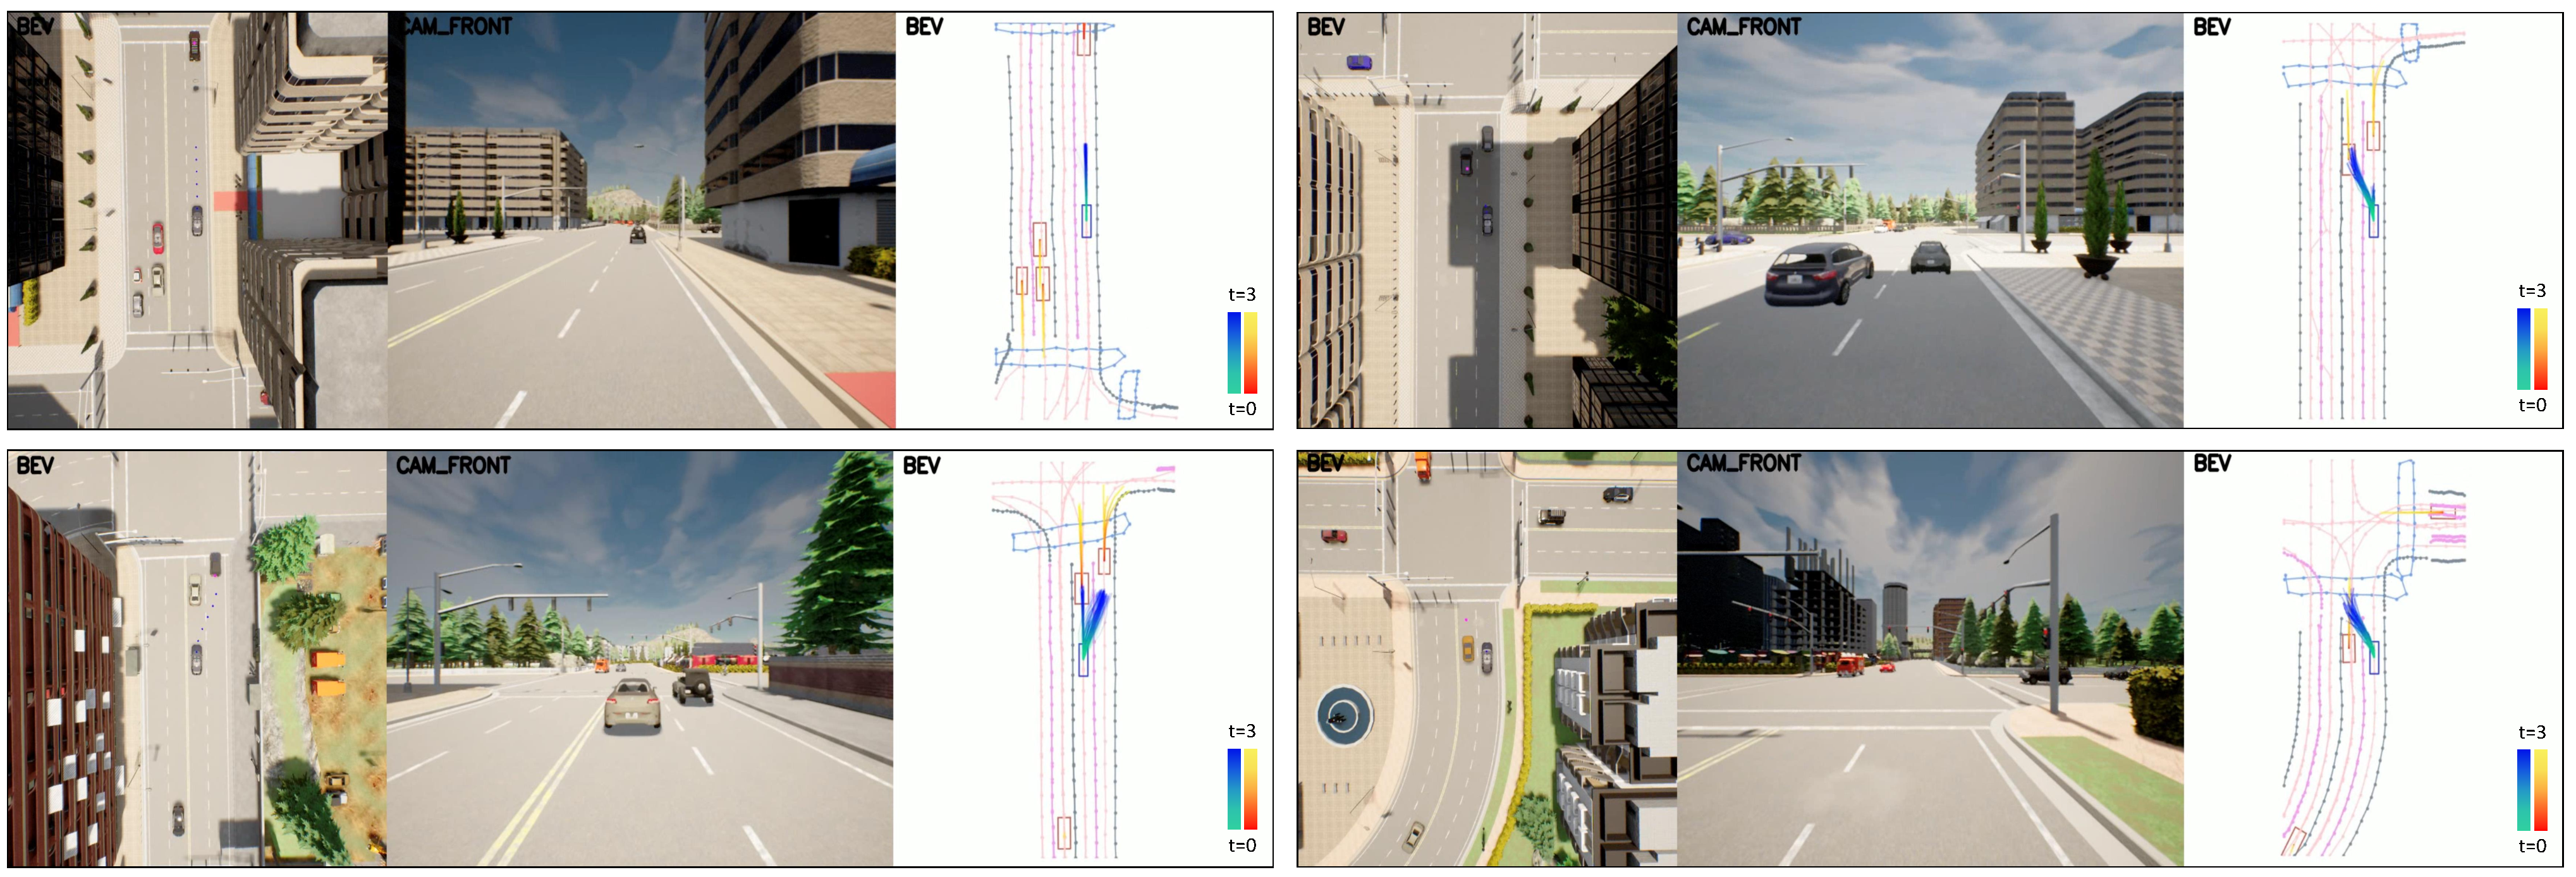
\includegraphics[width=1\textwidth]{fig/vis.pdf} % Reduce the figure size so that it is slightly narrower than the column.
}
% \vspace{-2mm}
\caption{\thename{}在CARLA Town05 Long基准上的定性结果。}
\vspace{-2mm}
\label{fig:vis}
\end{figure}


\boldparagraph{关键模块。}
表~\ref{tab:design}展示了\thename{}关键模块的消融实验，训练中使用了5万个驾驶演示片段。没有分布损失提供的专家驾驶行为监督（ID 1），模型在规划准确率上表现较差。冲突损失提供了关键的驾驶先验信息，因此移除它（ID 2）同样影响模型的规划准确率。场景令牌将重要的场景元素编码为高维特征，规划令牌与场景令牌交互以学习驾驶场景的动态和静态信息。当缺少任何类型的场景令牌时，模型的规划性能都会受到影响（ID 3-ID 6）。当模型包含上述所有设计时（ID 7），达到最佳规划性能。

\vspace{-1mm}
\boldparagraph{规划鲁棒性。}
基于自车20米范围内的动态智能体数量，将交通密度分为低（<5）、中（5–10）和高（>10），并在不同规划方式和密度级别下评估性能（表~\ref{tab:density}）。对于确定性规划，遵循常见做法~\citep{vad}将VADv2的规划头修改为直接回归未来轨迹的MLP。结果表明，概率规划始终优于确定性规划。此外，概率规划在不同密度场景下保持稳定性能，而确定性规划则表现出明显的性能下降。这些发现凸显了概率规划范式的有效性和鲁棒性。更多实验和消融见附录~\ref{sec:appendix}。


% \vspace{-1mm}
\subsection{可视化}
图~\ref{fig:vis}展示了\thename{}的定性结果。左上图显示不同驾驶速度下的多模态规划轨迹。右上图展示了向前蠕行和向左变道。左下图展示了路口处右变道场景，同时预测了临时直行和立即变道轨迹。右下图描述了目标车道有车辆时的变道情况，\thename{}生成了多条合理轨迹。


\vspace{-1mm}
\section{结论与局限性}
\vspace{-1mm}
\label{sec:conclusion}
本文提出了\thename{}——一个基于概率规划的端到端驾驶模型。它在CARLA仿真器中稳定运行，取得了最先进的闭环性能，显著优于现有方法。在NAVSIM和基于3DGS基准上的全面实验进一步证明了其在复杂驾驶场景中的有效性和鲁棒性。该概率规划范式的可行性得到了初步验证。

目前，仿真器和基于3DGS的闭环环境仍存在局限性，如智能体行为简单和场景真实感不足，这可能会限制VADv2的性能。在未来的工作中，计划探索如何利用大规模专家驾驶数据进一步提升规划性能，并弥合仿真与真实部署之间的差距。


\section*{致谢}
本工作得到国家自然科学基金（NSFC No. 62276108）的资助。


\bibliography{iclr2026_conference}
\bibliographystyle{iclr2026_conference}

\newpage

\appendix
\section{附录}
\label{sec:appendix}


\begin{table}[t]
\centering
\begin{minipage}{0.49\linewidth}
% \renewcommand{\tabcolsep}{8.0pt}
\caption{Town05 Short上的闭环结果。}
% \vspace{2mm}
\centering
\resizebox{0.7\linewidth}{!}{
\begin{tabular}{lccc}
\toprule
\multirow{2}{*}{方法} & \multirow{2}{*}{模态} & \multirow{2}{*}{DS $\uparrow$} & \multirow{2}{*}{RC $\uparrow$} \\
 & & & \\
\midrule
CILRS & C & 7.5 & 13.4 \\
LBC & C & 31.0 & 55.0 \\
Transfuser & C+L & 54.5 & 78.4 \\
ST-P3 & C & 55.1 & 86.7 \\
VAD & C & 64.3 & 87.3 \\
LeapVAD & C & 88.2 & 99.5 \\
\thename{} & C & 89.7 & 93.0 \\
\bottomrule
\end{tabular}
}
% \vspace{-1mm}
\label{tab:town05short}
\end{minipage}
\hfill
\begin{minipage}{0.49\linewidth}
\caption{词表大小的消融实验。}
% \vspace{2mm}
\centering
% \renewcommand{\tabcolsep}{8.0pt}
\resizebox{0.98\linewidth}{!}{
\begin{tabular}{ccccccc}
\toprule
\multirow{2}{*}{大小}   & \multicolumn{3}{c}{L2 (m) $\downarrow$} & \multicolumn{3}{c}{碰撞率 (\%) $\downarrow$} \\
  & 1s & 2s & 3s & 1s & 2s & 3s  \\
\midrule
256 & 0.110 & 0.207 & 0.337 & 0.000 & 0.019 & 0.057 \\
512 & 0.099 & 0.189 & 0.313 & 0.000 & 0.022 & 0.045\\
1024 & 0.093 & 0.175 & 0.293 & 0.000 & 0.020 & 0.044\\
2048 &0.088 & 0.173 & 0.294 & 0.000 & 0.017 & 0.041\\
4096 & 0.082 & 0.169 & 0.290 & 0.000 & 0.010 & 0.039 \\
\bottomrule
\end{tabular}
}
\label{tab:voca_size}
\end{minipage}
\end{table}


\begin{table}[t]
\centering
\begin{minipage}{0.49\linewidth}
\caption{训练片段数量的消融实验。}
% \vspace{2mm}
\centering
% \renewcommand{\tabcolsep}{6.0pt}
\resizebox{0.98\linewidth}{!}{
\begin{tabular}{ccccccc}
\toprule
\multirow{2}{*}{数量}  & \multicolumn{3}{c}{L2 (m) $\downarrow$} & \multicolumn{3}{c}{碰撞率 (\%) $\downarrow$} \\
  & 1s & 2s & 3s & 1s & 2s & 3s  \\
\midrule
$1\times10^5$ & 0.121 & 0.264 & 0.461 & 0.015 & 0.061 & 0.107\\
$3\times10^5$ & 0.082 & 0.169 & 0.290 & 0.000 & 0.010 & 0.039 \\
$1\times10^6$ & 0.073 & 0.153 & 0.267 & 0.000 & 0.008 & 0.027 \\
$3\times10^6$ & 0.072 & 0.133 & 0.225 & 0.000 & 0.000 & 0.007\\
\bottomrule
\end{tabular}
}
\label{tab:demonstration_amount}
\end{minipage}
\hfill
\begin{minipage}{0.49\linewidth}
\caption{规划方式的消融实验。}
% \vspace{2mm}
% \renewcommand{\tabcolsep}{5.0pt}
\centering
\resizebox{0.98\linewidth}{!}{
\begin{tabular}{l|cccc}
\toprule
\multirow{2}{*}{规划方式}  & \multirow{2}{*}{DS $\uparrow$} & \multirow{2}{*}{RC $\uparrow$}  & L2(m) & 碰撞率(\%)  \\
 & & & @3s$\downarrow$  & @3s$\downarrow$\\
\midrule
确定性 & 74.6 & 95.1 & 0.223 & 0.006\\
概率 & 85.1 & 98.4 & 0.225 & 0.007\\
\bottomrule
\end{tabular}
}
\label{tab:modeling}
\end{minipage}
\end{table}

\begin{table*}
\vspace{-1mm}
\caption{不同词表采样策略的离散化误差与性能消融实验。}
% \vspace{-1mm}
\small
\centering
\resizebox{0.99\textwidth}{!}{
\setlength\tabcolsep{5pt}
\begin{tabular}{lccccccccc}
\toprule
策略 & 平均L2 $\downarrow$ & 最大L2 $\downarrow$ & NC $\uparrow$ & DAC $\uparrow$ & TTC $\uparrow$ & Comf $\uparrow$ & EP $\uparrow$ & PDMS $\uparrow$ \\
\midrule
k-means & 0.132 & 0.217 & 97.9 & 97.2 & 94.5 & 100 & 81.9 & 89.0 \\
K-disks & 0.128 & 0.204 & 98.1 & 97.3 & 94.8 & 100 & 82.2 & 89.1 \\
nuScenes & 0.116 & 0.212 & 98.2 & 97.1 & 95.4 & 100 & 82.5 & 89.1 \\
FTS & 0.102 & 0.181 & 98.3 & 97.6 & 95.1 & 100 & 82.3 & 89.3 \\
\bottomrule
\end{tabular}
}
% \vspace{-2pt}
\label{tab:sampling}
% \vspace{-2mm}
\end{table*}


\subsection{Town05 Short基准上的闭环结果}
在表~\ref{tab:town05short}中总结了VADv2在Town05 Short基准上的结果。该基准评估特定驾驶行为，包括密集交通中的变道和路口前的变道。VADv2取得了最高的DS分数，而LeapVAD虽然RC更高但DS较低，表明违规更多。总体而言，这些结果凸显了\thename{}在挑战性场景中强大而可靠的驾驶能力。


\subsection{更多消融研究}
\boldparagraph{词表大小。} 表~\ref{tab:voca_size}展示了词表大小的消融实验。随着词表增大，L2和碰撞指标均改善。更大的词表能够以更小的离散化误差更好地表示动作空间。


\boldparagraph{训练片段数量。}
表~\ref{tab:demonstration_amount}是用于训练端到端模型的驾驶演示片段数量的消融实验。如预期，随着数据量增加，模型在L2和碰撞指标上表现更好。


\boldparagraph{概率 vs 确定性。}
Town05 Long基准上的消融结果（表~\ref{tab:modeling}）表明，确定性和概率规划在开环评估中表现相似。而在闭环设置下，概率规划取得显著更好的稳定性和性能，确定性规划则难以应对规划不确定性。


\begin{table}[t]
\centering
\begin{minipage}[t]{0.48\textwidth}
\captionof{table}{真实世界基于3DGS验证数据集的更多详细统计。}
% \vspace{2mm}
% \renewcommand{\tabcolsep}{5.0pt}
\centering
\resizebox{0.99\linewidth}{!}{
\begin{tabular}{lcc}
\toprule
场景 & 类别 & 占比 \\
\midrule
晴天 & 天气 & 74.78\% \\
夜间和雨天 & 天气 & 25.22\% \\
拥挤道路 & 精细行为 & 6.23\% \\
狭窄道路 & 精细行为 & 6.82\% \\
路口 & 精细行为 & 38.58\% \\
切入 & 交互场景 & 9.79\% \\
人行横道 & 交互场景 & 9.20\% \\
\bottomrule
\end{tabular}
}
\label{tab:dataset2}
\end{minipage}
\hfill
\begin{minipage}[t]{0.48\textwidth}
\centering
\captionof{figure}{CARLA Town05基准上规划词表的可视化。}
\resizebox{0.9\linewidth}{!}{
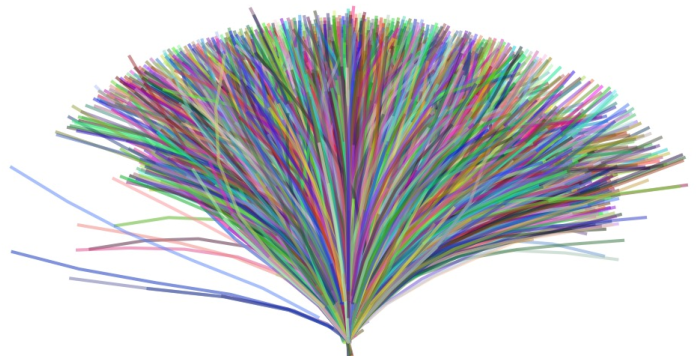
\includegraphics[width=1\textwidth]{fig/vocab.pdf}
}
\vspace{2mm}
\label{fig:vocab}
\end{minipage}
\end{table}


\begin{table*}[h]
\caption{基于3DGS基准的更多评估细节。}
\centering
{
\begin{tabular}{lccccc}
\toprule
方法 & 参考文献 & 参数量 & 延迟 & 碰撞率 (\%) & 平台 \\
\midrule
TransFuser & TPAMI 22 & 0.36B & 118ms & 0.320 & RTX 4090   \\
VAD & ICCV 23 & 0.36B & 118ms & 0.335 & RTX 4090   \\
GenAD & ECCV 24 & 0.38B & 121ms & 0.341 & RTX 4090   \\
VADv2 & 本文 & 0.40B & 125ms & 0.270 & RTX 4090   \\
\bottomrule
\end{tabular}
}
\label{tab:infer}
\end{table*}

\boldparagraph{词表采样。}
在表~\ref{tab:sampling}中，报告了不同词表采样策略的离散误差和规划性能。对于NAVSIM中的每个训练样本，选择L2距离最小的词表轨迹，然后测量每时间步的L2误差。同时计算平均和最大L2误差并在所有样本上取平均。

不同策略之间的差异较小，最远轨迹采样（FTS）取得了最佳的动作空间覆盖和最强的结果。同时通过从nuScenes训练集中采样轨迹构建词表并在NAVSIM上评估，性能保持可比，表明VADv2能够有效跨场景泛化。

\subsection{基于3DGS基准的更多评估细节}

表~\ref{tab:dataset2}展示了数据集中多样且具有挑战性的测试场景，支持更鲁棒的评估。同时在不同天气条件下评估基于3DGS的重建质量，晴天、雨天和夜间场景的PSNR（峰值信噪比）指标分别达到29.5、28.8和28.2，展现了领先的性能水平。

表~\ref{tab:infer}报告了TransFuser和VAD等基线方法的推理延迟、模型参数和硬件平台。为公平比较规划性能，所有方法使用相同的感知骨干网络，因此延迟差异主要来自规划模块设计。虽然VADv2的规划词表增加了一些开销，其延迟仍与其他基线相当，并显著改善了主要的碰撞率指标。

表~\ref{tab:dataset1}提供了真实世界数据集的额外细节并与主流基准进行比较。nuScenes以直行场景为主，NAVSIM包含更多转弯但数据量有限，而本数据集在规模和场景多样性方面均脱颖而出。


\subsection{LLM使用声明}
本文仅使用LLM进行语法检查和写作润色，作者对所有内容承担全部责任。

\begin{table*}[b]
\vspace{-2mm}
\caption{真实世界基于3DGS数据集的定量分析。}
\vspace{-1mm}
\centering
\resizebox{0.8\linewidth}{!}{
\setlength\tabcolsep{8pt}
\begin{tabular}{lcccc}
\toprule
数据集 & 时长 & 环境 & 直行 & 转弯 \\
\midrule
nuScenes & 5.55h & 城市 & 92.80\% & 7.20\% \\
NAVSIM & 120h & 城市 & 66.40\% & 33.60\% \\
本文 & 2000h & 城市、高速、乡村 & 52.50\% & 47.50\% \\
\bottomrule
\end{tabular}
}
\label{tab:dataset1}
\end{table*}

\end{document}
